\chapter{Evaluation}
\label{ch:evaluation}
The evaluation chapter describes the experiment setup and the results.

\section{Dataset}
The dataset consists of data from the Flickr API \footnote{\url{https://www.flickr.com/services/api/}}.
Flicker provides an API enpoint which containts data of the latest images.
As the API limits the number of requests per hour, the data had to be collected over an extended period of time.
The test data was gathered from this endpoint over a time period of about 4 weeks.

The internal representation in Elasticsearch of the data from Flickr can be seen in appendix \ref{ap:flickr-data}.
This data contains 115,105 photos and 298,962 tags, and the photo index takes up 152.3 MB in Elasticsearch.
Dynamic mapping was used for defining the fields for the internal representation in Elasticsearch.
A single index called \textit{photos} was used to hold the photo data.

\section{Experimental Setup}

The experiment setup consists of a client, a web server and a search engine.
Figure \ref{fig:experiment-setup} illustrates the experiment setup.
The client was a NodeJS script sending requests to the web server.

\begin{figure}[h!]
  \centering \includegraphics[width=0.9\linewidth]{img/experiment_setup.png}
  \caption{Experiment setup}
  \label{fig:experiment-setup}
\end{figure}

Elasticsearch's configuration was set to default settings,
except the memory heap size was changed to 4GB to make sure the search engine had sufficient memory.

\subsection{Hardware}
The experiment were conducted on a desktop computer with the specification described in table \ref{tbl:hardware}.

\begin{table}[h]
    \centering
    \begin{tabular}{c|c}
      \textbf{Component} & \textbf{Model} \\ \hline
      CPU       & Intel Core i5-4670 3.4 GHz x 4        \\ \hline
      RAM       & Crucial BallistixSport 2x8GB 1600 MHz \\ \hline
      SSD       & OCZ Vertex 4 256 GB                   \\ \hline
    \end{tabular}
    \caption{Hardware components of the computer running the experiments}
    \label{tbl:hardware}
\end{table}

\section{Results}
Measuring document relevance from users were never done as the main focus was latency and scaleability.

Latency was measure from the webserver recieved the request, to the server responded the user's request.
The round trip time from the webserver to the user is not taken into account.

As the web server and the search engine is on the same physical machine the round trip times are minimal.
However, in practice round trip times is often an important factor.

Figure \ref{fig:baseline} displays results from queries without query expansion.
The results without query expansion is used as a baseline,
to establish how much impact query expansion has on the respons times.

\begin{table}[h]
    \centering
    \begin{tabular}{c|l|l}
    Concurrent requests & Average (ms) & Median (ms) \\ \hline
    1                   & 8            & 7           \\ \hline
    5                   & 13           & 13          \\ \hline
    10                  & 20           & 20          \\ \hline
    15                  & 28           & 28          \\ \hline
    20                  & 34           & 35          \\ \hline
    30                  & 49           & 50          \\ \hline
    40                  & 63           & 63          \\ \hline
    \textbf{50}         & \textbf{73}  & \textbf{74} \\ \hline
    100                 & 123          & 115         \\ \hline
    150                 & 260          & 226         \\ \hline
    \end{tabular}
    \caption{Response times without query expansion}
    \label{tbl:baseline}
\end{table}

\begin{table}[h]
    \centering
    \begin{tabular}{c|l|l}
     Concurrent requests & Average (ms) & Median (ms) \\ \hline
    1                    & 16           & 14          \\ \hline
    5                    & 29           & 28          \\ \hline
    10                   & 49           & 49          \\ \hline
    \textbf{15}          & \textbf{74}  & \textbf{69} \\ \hline
    \textbf{20}          & \textbf{97}  & \textbf{96} \\ \hline
    30                   & 183          & 199         \\ \hline
    40                   & 219          & 198         \\ \hline
    50                   & 249          & 242         \\ \hline
    100                  & 476          & 428         \\ \hline
    150                  & 731          & 717         \\ \hline
    \end{tabular}
    \caption{Response times with query expansion}
    \label{tbl:query-expansion}
\end{table}

\begin{table}[h]
    \centering
    \begin{tabular}{c|l|l}
     Number of top-k documents & Average (ms) & Median (ms) \\ \hline
    10                         & 49           & 49          \\ \hline
    15                         & 56           & 51          \\ \hline
    20                         & 54           & 53          \\ \hline
    30                         & 57           & 53          \\ \hline
    40                         & 57           & 54          \\ \hline
    50                         & 58           & 56          \\ \hline
    100                        & 64           & 62          \\ \hline
    200                        & 76           & 72          \\ \hline
    \end{tabular}
    \caption{Response times while changing number of top-k documents}
    \label{tbl:query-expansion-topk}
\end{table}


\section{Discussion}
Figure \ref{fig:sequence-diagram-search-master} shows the sequence diagram for Rudihagen's query expansion solution using KL.
On the figure 4 round trips are required from the webserver to the database and the search engine.
The implementation discussed in Chapter \ref{ch:approach} describes a solution to decrease the number of round trips from 4 to 2.
In Chapter \ref{ch:evaluation} the performance is greatly increased.

\begin{figure}[h!]
\centering 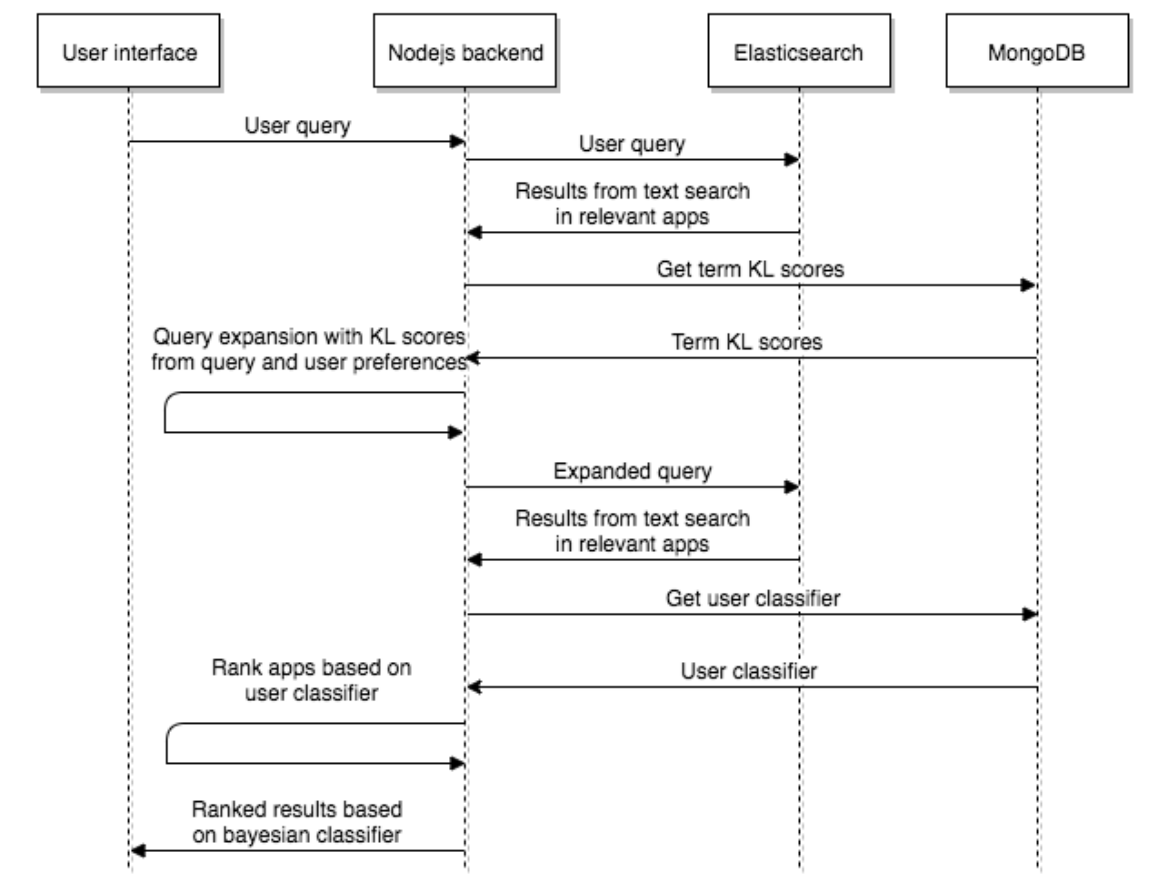
\includegraphics[width=0.9\linewidth]{img/sequence-diagram-search-master-thesis.png}
\caption{Sequence diagram from Rudihagen's master thesis implementation of query expansion using KL \cite[p. 37]{master-thesis}.}
\label{fig:sequence-diagram-search-master}
\end{figure}

Even though the latency was greatly reduced there are a few disclamers.
Firstly both the webserver and the search engine ran on the same computer.
As a result the round trip time was almost negligible, which is often not the case in a real world environment.
To give more realistic measurements, the solution should be tested on a cloud solution where the webserver and the search engine doesn't run on the same physical server.
